%%%%%%%%%%%%%%%%%%%%%%%%%%%%%%%%%%%%%%%%%
% Beamer Presentation
% LaTeX Template
% Version 1.0 (10/11/12)
%
% This template has been downloaded from:
% http://www.LaTeXTemplates.com
%
% License:
% CC BY-NC-SA 3.0 (http://creativecommons.org/licenses/by-nc-sa/3.0/)
%
%%%%%%%%%%%%%%%%%%%%%%%%%%%%%%%%%%%%%%%%%

%------------------------------------------------------------------------------------------------
% PACKAGES AND THEMES
%------------------------------------------------------------------------------------------------

\documentclass[table, xcolor = {dvipsnames}, 9pt]{beamer}
\usepackage{tikz}
\usetikzlibrary{calc}
\usetikzlibrary{positioning}
\usetikzlibrary{arrows.meta}
\usetikzlibrary{external}
\mode<presentation> {

\usetheme{default}
\usetheme{metropolis}
\usecolortheme{seagull}
\usefonttheme{professionalfonts}
}

\usepackage{graphicx} % Allows including images
\usepackage{booktabs} % Allows the use of \toprule, \midrule and \bottomrule in tables
\usepackage{float}
\usepackage{tikz}
\usepackage{multirow}
\usepackage{natbib}
\usepackage{hyperref}
\usepackage{diagbox}
\usepackage{makecell}
\usepackage{xparse}
\usepackage{subfig}
\usepackage{amsmath}
\usepackage{amsfonts,amsthm,amsmath,amssymb}
\usepackage{bbm}
\usepackage{bm}
\usepackage{empheq}
\usepackage{pgfplots}
\usepackage{animate}
\usepgfplotslibrary{colorbrewer}
\pgfplotsset{compat=1.17}

\newcommand\mybox[2][]{\tikz[overlay]\node[fill=lightgray,inner sep=2pt, anchor=text, rectangle, rounded corners=1mm,#1] {#2};\phantom{#2}}
\hypersetup{unicode=true,
            bookmarksnumbered=true,
            bookmarksopen=true,
            bookmarksopenlevel=2,
            breaklinks=false,
            pdfborder={0 0 1},
            hypertexnames=false,
            pdfstartview={XYZ null null 1}}
\usepackage{xcolor}
% R code listing style (matches the course's R-code slides)
\usepackage{listings}
\definecolor{codegreen}{rgb}{0,0.6,0}
\definecolor{codegray}{rgb}{0.5,0.5,0.5}
\definecolor{codepurple}{rgb}{0.58,0,0.82}
\definecolor{backcolour}{rgb}{0.95,0.95,0.92}
\lstdefinestyle{Rstyle}{
    language=R,
    backgroundcolor=\color{backcolour},
    commentstyle=\color{codegreen},
    keywordstyle=\color{magenta},
    stringstyle=\color{codepurple},
    basicstyle=\ttfamily\footnotesize,
    breakatwhitespace=false,
    breaklines=true,
    keepspaces=true,
    showspaces=false,
    showstringspaces=false,
    showtabs=false,
    tabsize=2
}
\newcommand\myheading[1]{%
  \par\bigskip
  {\Large\bfseries#1}\par\smallskip}
\newcommand\given[1][]{\:#1\vert\:}
\theoremstyle{plain}
\newtheorem{thm}{Theorem}
\newtheorem{prop}{Proposition\thisthmnumber}
\newtheorem{lem}{Lemma\thisthmnumber}
\newtheorem{cor}{Corollary}
\newtheorem{defin}{Definition}
\newtheorem{algo}{Algorithm}
\newcommand*\diff{\mathop{}\!\mathrm{d}}
\newcommand*\Diff[1]{\mathop{}\!\mathrm{d^#1}}
\newcommand{\bh}[1]{{\color{blue}{#1}}}
\newcommand{\mh}[1]{{\color{magenta}{#1}}}
\newcommand{\thisthmnumber}{}
\newcommand{\tikzmark}[1]{\tikz[baseline,remember picture] \coordinate (#1) {};}
\newcommand*{\QEDA}{\hfill\ensuremath{\blacksquare}}%
\newcommand*{\QEDB}{\hfill\ensuremath{\square}}%
\DeclareMathOperator{\E}{\rm{E}}
\DeclareMathOperator{\R}{\mathbb{R}}
\DeclareMathOperator{\N}{\mathbb{N}}
\DeclareMathOperator{\Var}{\rm{Var}}
\DeclareMathOperator{\Cov}{\rm{Cov}}
\DeclareMathOperator{\Supp}{\rm{Supp}}
\DeclareMathOperator{\e}{\rm{e}}
\DeclareMathOperator{\F}{\mathcal{F}}
\DeclareMathOperator{\Z}{\mathcal{Z}}
\DeclareMathOperator{\logit}{\rm{logit}}
\DeclareMathOperator{\indep}{{\perp\!\!\!\perp}}
\DeclareMathOperator{\rank}{rank}
\DeclareMathOperator*{\argmin}{arg\,min}
\DeclareMathOperator*{\argmax}{arg\,max}
% Shorthands for the intention-to-treat effects used throughout
\newcommand{\ITTY}{\mathrm{ITT}_Y}
\newcommand{\ITTD}{\mathrm{ITT}_D}
\newcommand{\CACE}{\mathrm{CACE}}
% Estimators: hat over the letters only, subscript outside the hat
\newcommand{\hITTY}{\widehat{\mathrm{ITT}}_Y}
\newcommand{\hITTD}{\widehat{\mathrm{ITT}}_D}
%------------------------------------------------------------------------
% TITLE PAGE
%-----------------------------------------------------------------------
\pagestyle{empty}
\title[Effects within principal strata]{Noncompliance, Attrition, and Average Effects within Principal Strata} % The short title appears at the bottom of every slide, the full title is only on the title page

\author{Thomas Leavitt} % Your name
\institute[] % Your institution as it will appear on the bottom of every slide, may be shorthand to save space
{
\medskip
\textit{}
}
\date{June 23, 2026} % Date, can be changed to a custom date

\begin{document}

\begin{frame}
\titlepage % Print the title page as the first slide
\end{frame}

%------------------------------------------------------------------------
% PRESENTATION SLIDES
%------------------------------------------------------------------------
\section{Where we landed}

\begin{frame}[t]{So far: inference for the average effect}
\vfill
\begin{itemize} \vfill
\item \textbf{Estimand}: the ATE $\bar{\tau} = \bar{y}(1) - \bar{y}(0)$ \vfill
\item \textbf{Estimator}: Difference-in-Means $\hat{\tau}\left(\bm{Z}, \bm{Y}\right)$, treated mean $-$ control mean \vfill
\item Under CRA, \emph{whatever} the potential outcomes, $\E\left[\hat{\tau}\left(\bm{Z}, \bm{Y}\right)\right] = \bar{\tau}$ \vfill
\item Conservative variance $\Rightarrow$ standard error, test, confidence interval \vfill
\item Yesterday: \mh{covariance adjustment} $\Rightarrow$ added precision from baseline covariates \vfill
\item All of this assumed an \mh{ideal} experiment \vfill
\begin{itemize} \vfill
\item Every unit \emph{receives} its assigned treatment \vfill
\item Every unit's outcome is \emph{observed} \vfill
\end{itemize} \vfill
\end{itemize} \vfill
\end{frame}
%------------------------------------------------------------------------
\begin{frame}[t]{Today: two cracks in the ideal experiment}
\vfill
\begin{itemize} \vfill
\item \mh{Noncompliance}: assigned treatment $\neq$ treatment \emph{received} \vfill
\begin{itemize} \vfill
\item Some assigned to treatment go untreated; some controls get treated \vfill
\end{itemize} \vfill
\item \mh{Attrition}: some outcomes are \emph{missing}, perhaps selectively \vfill
\begin{itemize} \vfill
\item Subjects drop out, refuse, cannot be found \vfill
\end{itemize} \vfill
\item Randomization governs \emph{assignment} --- not receipt or reporting \vfill
\item[] $\Rightarrow$ what changes is \mh{which causal effect we can identify} \vfill
\item Tools stay design-based; the \emph{estimand} narrows to a subpopulation \vfill
\end{itemize} \vfill
\end{frame}
%------------------------------------------------------------------------
\section{Four quantities, not two}

\begin{frame}[t]{Separate assignment, receipt, reporting, and outcome}
\vfill
\begin{itemize} \vfill
\item \textbf{Assignment} $Z_i$: what the \emph{randomizer} does ($1$ = treatment, $0$ = control) \vfill
\item \textbf{Receipt} $D_i$: the treatment the unit actually \emph{takes} \vfill
\item \textbf{Reporting} $R_i$: whether the outcome is \emph{observed} ($1$) or missing ($0$) \vfill
\item \textbf{Outcome} $Y_i$: the response of interest, when reported \vfill
\end{itemize} \vfill
\begin{itemize} \vfill
\item Ideal experiment: $D_i = Z_i$ and $R_i = 1$ for all $i$ \vfill
\item \mh{Only $\bm{Z}$ is randomized}; $D_i$, $R_i$, $Y_i$ are downstream behaviors \vfill
\end{itemize} \vfill
\end{frame}
%------------------------------------------------------------------------
\begin{frame}[t]{Receipt and reporting are potential outcomes too}
\vfill
\begin{itemize} \vfill
\item Receipt under each assignment: $d_i(1), d_i(0)$ --- \mh{fixed} attributes of unit $i$ \vfill
\item[] Observed receipt: $D_i = d_i(1) Z_i + d_i(0)\left(1 - Z_i\right)$ \vfill
\item Reporting under each assignment: $r_i(1), r_i(0)$ --- also fixed \vfill
\item[] Observed reporting: $R_i = r_i(1) Z_i + r_i(0)\left(1 - Z_i\right)$ \vfill
\item Outcome potential outcomes $y_i(1), y_i(0)$ as before; $\tau_i = y_i(1) - y_i(0)$ \vfill
\item \mh{Same logic as Day 3}: lowercase $=$ fixed potential outcomes, $\bm{Z}$ varies \vfill
\end{itemize} \vfill
\end{frame}
%------------------------------------------------------------------------
\section{Noncompliance: the CACE}

\begin{frame}[t]{Running example: the 1980 GOTV experiment}
\vfill
\begin{itemize} \vfill
\item Telephone get-out-the-vote experiment \citep{adamssmith1980} \vfill
\item $N = 2650$ registered voters; $n_1 = 1325$ assigned a call, $n_0 = 1325$ control \vfill
\item \textbf{Assignment} $Z_i$: randomized to receive an encouragement call \vfill
\item \textbf{Receipt} $D_i$: whether the voter was actually \emph{reached} by a caller \vfill
\item \textbf{Outcome} $Y_i$: whether the voter \emph{turned out} \vfill
\item \mh{One-sided noncompliance}: a control voter \emph{cannot} be reached ($d_i(0) = 0$) \vfill
\item Only $950$ of the $1325$ called were reached --- assignment $\neq$ receipt \vfill
\end{itemize} \vfill
\end{frame}
%------------------------------------------------------------------------
\begin{frame}[t]{The assignment acts on the outcome only through receipt}
\vfill
\begin{center}
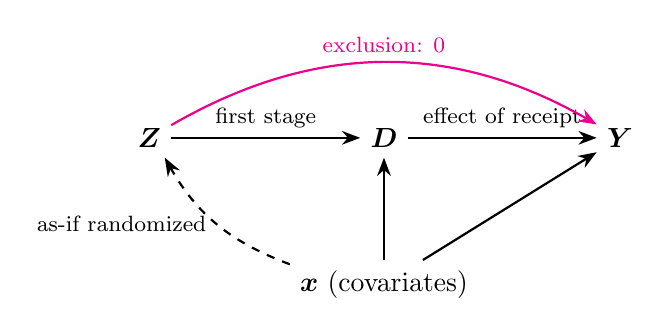
\begin{tikzpicture}[>=Stealth, node distance = 2.4cm, thick]
\node (Z) {$\bm{Z}$};
\node (D) [right = of Z] {$\bm{D}$};
\node (Y) [right = of D] {$\bm{Y}$};
\node (X) [below = 1.3cm of D] {$\bm{x}$ (covariates)};
\draw[->] (Z) -- node[above]{\footnotesize first stage} (D);
\draw[->] (D) -- node[above]{\footnotesize effect of receipt} (Y);
\draw[->, magenta] (Z) to[bend left = 30] node[above]{\footnotesize exclusion: $0$} (Y);
\draw[->] (X) -- (D);
\draw[->] (X) -- (Y);
\draw[->, dashed] (X) to[bend left = 20] node[left]{\footnotesize as-if randomized} (Z);
\end{tikzpicture}
\end{center}
\vfill
\begin{itemize} \vfill
\item \textbf{Target}: the effect of \mh{receipt} $\bm{D}$ on the outcome $\bm{Y}$ --- the $\bm{D} \to \bm{Y}$ arrow \vfill
\item[] \textbf{GOTV}: effect of actually being \emph{reached} on turning out to vote \vfill
\item Receipt $\bm{D}$ is \emph{not} randomized --- it is confounded by $\bm{x}$ \vfill
\item[] So a raw $D = 1$ vs.\ $D = 0$ contrast is \mh{not} the effect of $\bm{D}$ \vfill
\item Randomization severs $\bm{x} \to \bm{Z}$: assignment is \mh{independent} of the POs \vfill
\item \mh{Exclusion} (to come): the magenta arrow is $0$ --- $\bm{Z}$ hits $\bm{Y}$ only via $\bm{D}$ \vfill
\end{itemize} \vfill
\end{frame}
%------------------------------------------------------------------------
\begin{frame}[t]{Compliance principal strata}
\vfill
\begin{itemize} \vfill
\item Partition units by the pair $\left(d_i(0), d_i(1)\right)$ \vfill
\end{itemize}
\vfill
\begin{table}[H]
\centering
\begin{tabular}{c|c|l}
$z_i = 0$ & $z_i = 1$ & Principal stratum \\ \hline
$d_i(0) = 1$ & $d_i(1) = 1$ & \textit{Always-Taker} (AT) \\
$d_i(0) = 0$ & $d_i(1) = 1$ & \textit{Complier} (C) \\
$d_i(0) = 1$ & $d_i(1) = 0$ & \textit{Defier} (D) \\
$d_i(0) = 0$ & $d_i(1) = 0$ & \textit{Never-Taker} (NT) \\
\end{tabular}
\end{table}
\vfill
\begin{itemize} \vfill
\item \mh{Compliers} take the dose \emph{exactly when} assigned it \vfill
\item Proportions $\pi^{\textrm{AT}}, \pi^{\textrm{C}}, \pi^{\textrm{D}}, \pi^{\textrm{NT}}$ sum to $1$ \vfill
\end{itemize} \vfill
\end{frame}
%------------------------------------------------------------------------
\begin{frame}[t]{Each $\bm{Z}\times\bm{D}$ cell mixes two strata}
\vfill
\begin{itemize} \vfill
\item The observed cell tells us a \emph{pair}, never the stratum \vfill
\item Treated and took dose ($z_i = 1$, $D_i = 1$): \mh{C or AT} \vfill
\item Treated and no dose ($z_i = 1$, $D_i = 0$): NT or D \vfill
\item Control and took dose ($z_i = 0$, $D_i = 1$): AT or D \vfill
\item Control and no dose ($z_i = 0$, $D_i = 0$): C or NT \vfill
\item \textbf{GOTV}: one-sided $\Rightarrow$ no AT, no D $\Rightarrow$ only \mh{Compliers} and \mh{Never-Takers} \vfill
\end{itemize} \vfill
\end{frame}
%------------------------------------------------------------------------
\begin{frame}[t]{One-sided vs two-sided noncompliance}
\vfill
\begin{itemize} \vfill
\item \textbf{One-sided} (our GOTV running example): controls \emph{cannot} get the dose \vfill
\item[] $d_i(0) = 0$ for all \vfill
\item[] $\Rightarrow$ no Always-Takers and no Defiers \mh{by construction} \vfill
\item[] Anyone dosed when treated is a \mh{Complier} \vfill
\item[] Monotonicity $d_i(1) \geq d_i(0)$ holds \emph{automatically} \vfill
\item \textbf{Two-sided} (Albertson \& Lawrence: encouraged to \emph{watch} a program) \vfill
\item[] \citep{albertsonlawrence2009} \vfill
\item[] Some encouraged don't watch; some controls watch anyway \vfill
\item[] $\Rightarrow$ all four strata possible \vfill
\item[] No Defiers (monotonicity) is now an \mh{assumption}, not a fact \vfill
\end{itemize} \vfill
\end{frame}
%------------------------------------------------------------------------
\begin{frame}[t]{Three different effects of assignment}
\vfill
\begin{itemize} \vfill
\item \textbf{Reduced form} $\ITTY$: effect of \emph{assignment} on the outcome \vfill
\begin{equation*}
\ITTY = \bar{\tau} = \bar{y}(1) - \bar{y}(0), \qquad \hITTY = \hat{\tau}\left(\bm{Z}, \bm{Y}\right)
\end{equation*} \vfill
\item \textbf{First stage} $\ITTD$: effect of \emph{assignment} on receipt \vfill
\begin{equation*}
\ITTD = \bar{d}(1) - \bar{d}(0), \qquad \hITTD = \hat{\tau}\left(\bm{Z}, \bm{D}\right)
\end{equation*} \vfill
\item \textbf{CACE} $\tau^{\textrm{C}}$: effect of \emph{receipt} among Compliers \vfill
\item Both ITTs are \mh{safe} --- effects of the randomized $\bm{Z}$, estimable as on Day 4 \vfill
\item The CACE is the prize, but it is an effect of the \emph{non}-randomized $\bm{D}$ \vfill
\end{itemize} \vfill
\end{frame}
%------------------------------------------------------------------------
\begin{frame}[t]{Why not just compare the treated by receipt?}
\vfill
\begin{itemize} \vfill
\item Tempting \mh{per-protocol} contrast: $\bar{Y}_{D = 1} - \bar{Y}_{D = 0}$ \vfill
\item Receipt $\bm{D}$ is \emph{not} randomized --- the two $D$-groups are different \mh{types}: \vfill
\begin{itemize} \vfill
\item $D = 1$ (reached): all \mh{Compliers}, under treatment \vfill
\item $D = 0$ (not reached): \mh{Never-Takers} $+$ Compliers assigned control \vfill
\end{itemize} \vfill
\item So it compares Compliers against a Complier/Never-Taker \mh{mix} \vfill
\item \textbf{GOTV per-protocol}: $0.326 - 0.234 \approx \mh{+9.3}$ points (confounded) \vfill
\item \mh{Analyze as you randomized}: the ratio $\CACE = \ITTY/\ITTD$ \vfill
\end{itemize} \vfill
\end{frame}
%------------------------------------------------------------------------
\begin{frame}[t]{Per-protocol = a dose propensity that predicts outcomes}
\vfill
\begin{itemize} \vfill
\item Per-protocol treats $D$ as randomized --- but dose chances differ by unit \vfill
\item $\Pr(D_i = 1)$ is a \mh{type-dependent propensity}: \vfill
\begin{itemize} \vfill
\item Compliers $\Pr(D_i = 1) = \Pr(Z_i = 1) = n_1/N$; \; Never-Takers $0$ \vfill
\item Always-Takers $1$; \; Defiers $\Pr(Z_i = 0) = n_0/N$ \vfill
\end{itemize} \vfill
\item Type predicts the potential outcomes, so this propensity does too \vfill
\item[] $\Rightarrow$ $D = 1$ vs $D = 0$ compares units with \emph{different} POs: confounded \vfill
\item The strata-composition gap is just the \mh{degenerate} case of this \vfill
\end{itemize} \vfill
\end{frame}
%------------------------------------------------------------------------
\begin{frame}[t]{Assumptions for the CACE}
\vfill
\begin{itemize} \vfill
\item \textbf{A1 (SUTVA / non-interference).} Unit $i$'s $D, Y$ depend only on $z_i$ \vfill
\item[] $\Rightarrow$ just two potential outcomes per unit $\Rightarrow$ principal strata well-defined \vfill
\item \textbf{A2 (Exclusion).} $\bm{Z}$ affects $\bm{Y}$ only through $\bm{D}$: so $\tau_i = 0$ for AT, NT \vfill
\item \textbf{A3 (No Defiers / monotonicity).} $d_i(1) \geq d_i(0)$ for all $i$ $\Rightarrow$ $\pi^{\textrm{D}} = 0$ \vfill
\item[] Automatic under one-sided noncompliance \vfill
\item[] a genuine \emph{assumption} under two-sided \vfill
\item \textbf{A4 (Existence of Compliers).} $\pi^{\textrm{C}} > 0$ (a \mh{strong} instrument) \vfill
\item \mh{Identification} needs A1--A4; random assignment enters later, to \emph{estimate} \vfill
\end{itemize} \vfill
\end{frame}
%------------------------------------------------------------------------
\begin{frame}[t]{Estimand: the Complier Average Causal Effect}
\vfill
\begin{itemize} \vfill
\item \textbf{Estimand}:
\begin{equation*}
\CACE = \tau^{\textrm{C}} = \bar{y}^{\textrm{C}}(1) - \bar{y}^{\textrm{C}}(0)
\end{equation*} \vfill
\item Average effect of \emph{receiving} the treatment, \mh{among Compliers} \vfill
\item Compliers are a \mh{latent} subgroup: $\left(d_i(0), d_i(1)\right)$ is never both seen \vfill
\item[] We cannot \emph{list} the Compliers, so we cannot average over them directly \vfill
\item Under \mh{A1--A4}, no random assignment needed: $\CACE = \ITTY / \ITTD$ \vfill
\end{itemize} \vfill
\end{frame}
%------------------------------------------------------------------------
\begin{frame}[t]{The idea: trade a latent subgroup for whole-sample effects}
\vfill
\begin{itemize} \vfill
\item \textbf{Problem}: the CACE lives on a subgroup we \mh{cannot identify} \vfill
\item \textbf{Idea}: show $\CACE = \dfrac{\ITTY}{\ITTD}$, a ratio of effects on \mh{all $N$ units} \vfill
\item Neither $\ITTY$ nor $\ITTD$ refers to who is a Complier \vfill
\item[] Both are plain differences of means over the \emph{whole} sample \vfill
\item So we recover a \mh{subgroup} effect from two \mh{whole-sample} effects \vfill
\item[] $\Rightarrow$ no need to know \emph{which} units are Compliers \vfill
\item The identity is the engine; estimation (later) never finds a Complier \vfill
\end{itemize} \vfill
\end{frame}
%------------------------------------------------------------------------
\begin{frame}[t]{Proof, step 1: decompose $\ITTY$ over strata}
\vfill
\begin{itemize} \vfill
\item $\ITTY$ is the average individual effect: $\ITTY = \dfrac{1}{N}\sum_{i=1}^{N} \tau_i$ \vfill
\item Group the $N$ units by compliance type and sum \emph{within} each type: \vfill
\begin{align*}
\sum_{i=1}^{N} \tau_i = N^{\textrm{AT}} \tau^{\textrm{AT}} + N^{\textrm{C}} \tau^{\textrm{C}} + N^{\textrm{D}} \tau^{\textrm{D}} + N^{\textrm{NT}} \tau^{\textrm{NT}}
\end{align*} \vfill
\item[] $N^{\textrm{type}}$: count in that type; $\tau^{\textrm{type}}$: its average effect \vfill
\item Divide by $N$; each share is $N^{\textrm{type}}/N = \pi^{\textrm{type}}$: \vfill
\begin{align*}
\ITTY = \pi^{\textrm{AT}} \tau^{\textrm{AT}} + \pi^{\textrm{C}} \tau^{\textrm{C}} + \pi^{\textrm{D}} \tau^{\textrm{D}} + \pi^{\textrm{NT}} \tau^{\textrm{NT}}
\end{align*} \vfill
\item So far just an \mh{accounting identity} --- no assumptions yet \vfill
\item[] besides \textbf{A1 (SUTVA / non-interference)} \vfill
\end{itemize} \vfill
\end{frame}
%------------------------------------------------------------------------
\begin{frame}[t]{Proof, step 2: exclusion and no-Defiers prune the sum}
\vfill
\begin{itemize} \vfill
\item \textbf{Exclusion (A2)}: $\tau^{\textrm{AT}} = 0$ and $\tau^{\textrm{NT}} = 0$ \vfill
\begin{equation*}
\ITTY = \pi^{\textrm{C}} \tau^{\textrm{C}} + \pi^{\textrm{D}} \tau^{\textrm{D}}
\end{equation*} \vfill
\item \textbf{No Defiers (A3)}: $\pi^{\textrm{D}} = 0$ \vfill
\begin{equation*}
\ITTY = \mh{\pi^{\textrm{C}} \tau^{\textrm{C}}}
\end{equation*} \vfill
\item The reduced form is the Complier effect, \emph{diluted} by the Complier share \vfill
\end{itemize} \vfill
\end{frame}
%------------------------------------------------------------------------
\begin{frame}[t]{Proof, step 3: the first stage is the Complier share}
\vfill
\begin{itemize} \vfill
\item $\ITTD$ is the average first stage: $\ITTD = \dfrac{1}{N}\sum_{i=1}^{N} \left(d_i(1) - d_i(0)\right)$ \vfill
\item For each unit $d_i(1) - d_i(0) \in \{-1, 0, 1\}$: \vfill
\begin{itemize} \vfill
\item $+1$ for Compliers, $-1$ for Defiers, $0$ for Always- and Never-Takers \vfill
\end{itemize} \vfill
\item Summing, the $\pm 1$'s count Compliers against Defiers: \vfill
\begin{align*}
\sum_{i=1}^{N} \left(d_i(1) - d_i(0)\right) = N^{\textrm{C}} - N^{\textrm{D}}
\end{align*} \vfill
\item Divide by $N$; each count becomes a share $N^{\textrm{type}}/N = \pi^{\textrm{type}}$: \vfill
\begin{align*}
\ITTD = \frac{1}{N}\left(N^{\textrm{C}} - N^{\textrm{D}}\right) = \pi^{\textrm{C}} - \pi^{\textrm{D}}
\end{align*} \vfill
\item \textbf{No Defiers (A3)}: $\ITTD = \mh{\pi^{\textrm{C}}}$ \vfill
\end{itemize} \vfill
\end{frame}
%------------------------------------------------------------------------
\begin{frame}[t]{Proof, step 4: the ratio is the CACE}
\vfill
\begin{itemize} \vfill
\item Take the ratio of steps 2 and 3: \vfill
\begin{equation*}
\frac{\ITTY}{\ITTD} = \frac{\pi^{\textrm{C}} \tau^{\textrm{C}}}{\pi^{\textrm{C}}} = \tau^{\textrm{C}} = \CACE
\end{equation*} \vfill
\item \mh{Existence of Compliers (A4)}: $\pi^{\textrm{C}} > 0$ makes the division legal \vfill
\item Each assumption pulled its weight: \vfill
\begin{itemize} \vfill
\item A2 emptied the AT/NT terms; A3 emptied the D term; A4 let us divide \vfill
\end{itemize} \vfill
\item \mh{No random assignment used}: an identity among \emph{fixed} potential outcomes \vfill
\item[] Random assignment enters only to \emph{estimate} $\ITTY$ and $\ITTD$ (next) \vfill
\end{itemize} \vfill
\end{frame}
%------------------------------------------------------------------------
\begin{frame}[t]{The Wald estimator: intuition then formula}
\vfill
\begin{itemize} \vfill
\item \mh{Intuition}: assignment moves only the Compliers' dose \vfill
\begin{itemize} \vfill
\item It buys an outcome shift $\ITTY$ by moving a \emph{fraction} $\pi^{\textrm{C}}$ of doses \vfill
\item Undo the dilution: divide the shift by the fraction moved \vfill
\end{itemize} \vfill
\item \textbf{Wald / Bloom estimator} \citep{bloom1984, angristetal1996}: \vfill
\begin{equation*}
\widehat{\CACE} = \frac{\hITTY}{\hITTD} = \frac{\hat{\tau}\left(\bm{Z}, \bm{Y}\right)}{\hat{\tau}\left(\bm{Z}, \bm{D}\right)}
\end{equation*} \vfill
\item $\hITTY, \hITTD$ are whole-sample Difference-in-Means --- \mh{no Complier labels} \vfill
\item[] Recovers the subgroup effect \emph{without identifying a single Complier} \vfill
\end{itemize} \vfill
\end{frame}
%------------------------------------------------------------------------
\begin{frame}[fragile]{The Wald estimator in \texttt{R}}
\begin{lstlisting}[style=Rstyle, basicstyle=\ttfamily\tiny, frame=single]
diff_in_means <- function(z, y) mean(y[z == 1]) - mean(y[z == 0])

itt_y_hat <- diff_in_means(z = z_obs, y = y_obs)   # reduced form ~ 0.0581
itt_d_hat <- diff_in_means(z = z_obs, y = d_obs)   # first stage  ~ 0.7170
cace_hat  <- itt_y_hat / itt_d_hat                 # Wald ratio   ~ 0.0811
\end{lstlisting}
\vfill
\begin{itemize} \vfill
\item Apply the \emph{same} estimator to $\bm{Y}$ and to $\bm{D}$, then divide \vfill
\item \mh{Consistent}: with a large experiment, $\widehat{\CACE}$ is close to $\CACE$ w.h.p. \vfill
\item Not generally \emph{unbiased} --- expectation of a ratio $\neq$ ratio of expectations \vfill
\end{itemize}
\end{frame}
%------------------------------------------------------------------------
\section{Adams \& Smith: estimate the effects}

\begin{frame}[t]{Exercise: the GOTV data}
\vfill
\begin{itemize} \vfill
\item GOTV experiment \citep{adamssmith1980}: $N = 2650$, $n_1 = n_0 = 1325$ \vfill
\item \mh{One-sided}: no control voter is reached \vfill
\item \textbf{Reached} ($D = 1$): $950$ of $1325$ telephoned; $0$ controls \vfill
\item \textbf{Voted} ($Y = 1$): $392$ of $1325$ telephoned; $315$ of $1325$ controls \vfill
\item Among the $950$ reached, $310$ voted \vfill
\item All counts and turnout rates appear in the figure (next) \vfill
\end{itemize} \vfill
\end{frame}
%------------------------------------------------------------------------
\begin{frame}{The GOTV data, visualized}
\begin{figure}[H]
\centering
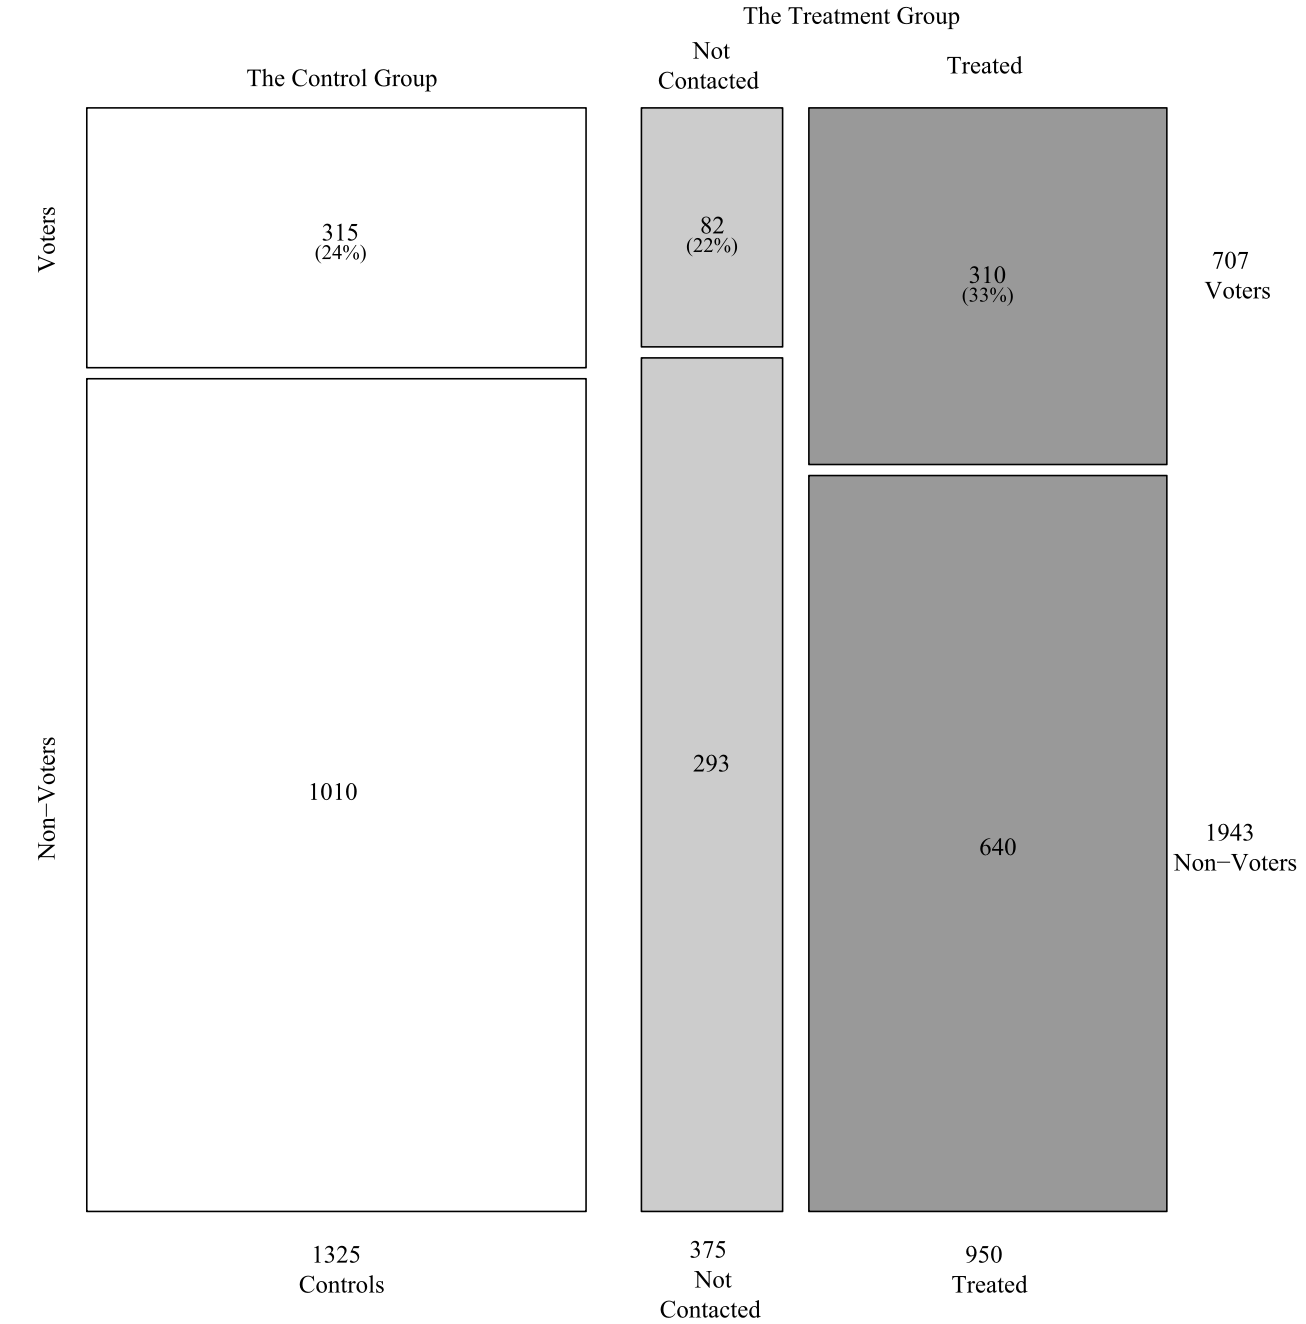
\includegraphics[height=0.78\textheight]{figures/hansen_bowers_2009.png}
\end{figure}
\vspace{-0.6em}
\centering \footnotesize Block areas $\propto$ group sizes; shaded $=$ voters \citep{hansenbowers2009} \normalsize
\end{frame}
%------------------------------------------------------------------------
\begin{frame}[t]{Exercise: your tasks}
\vfill
\textbf{Work in pairs. Using only the table:}
\begin{enumerate} \vfill
\item Identify the assignment, the receipt, and the outcome \vfill
\item Which compliance strata can be present? Which are ruled out, and why? \vfill
\item State the exclusion restriction here. Is it plausible? \vfill
\item Estimate $\hITTY$ (reduced form) \vfill
\item Estimate $\hITTD$ (first stage) \vfill
\item Estimate $\widehat{\CACE}$ and interpret it; name its population \vfill
\end{enumerate}
\vfill
\vfill
\end{frame}
%------------------------------------------------------------------------
\begin{frame}[t]{Solution: structure and strata}
\vfill
\begin{itemize} \vfill
\item \textbf{Assignment} $Z$: randomized to a call; \textbf{Receipt} $D$: reached \vfill
\item[] \textbf{Outcome} $Y$: voted \vfill
\item One-sided $\Rightarrow$ $d_i(0) = 0$ for all $\Rightarrow$ \mh{no Always-Takers, no Defiers} \vfill
\item Only \mh{Compliers} (reached when called) and \mh{Never-Takers} (never reached) \vfill
\item \textbf{Exclusion}: being \emph{called but not reached} does not change turnout \vfill
\begin{itemize} \vfill
\item Plausible: an unanswered call leaves no message, no information \vfill
\end{itemize} \vfill
\item \textbf{Compliers exist}: clearly, $950$ of $1325$ were reached \vfill
\end{itemize} \vfill
\end{frame}
%------------------------------------------------------------------------
\begin{frame}[t]{Solution: the three estimates}
\vfill
\begin{itemize} \vfill
\item \textbf{Reduced form}: $\hITTY = \dfrac{392}{1325} - \dfrac{315}{1325} = 0.296 - 0.238 = \mh{0.058}$ \vfill
\item \textbf{First stage}: $\hITTD = \dfrac{950}{1325} - \dfrac{0}{1325} = \mh{0.717}$ \vfill
\item \textbf{Wald ratio}: $\widehat{\CACE} = \dfrac{0.058}{0.717} = \mh{0.081}$ \vfill
\item \mh{Interpretation}: actually \emph{reaching} a voter raised turnout by $\approx 8.1$ points \vfill
\item \mh{Population}: Compliers --- voters reachable \emph{because} called \vfill
\item Contrast the confounded per-protocol $+9.3$: the CACE is design-based \vfill
\end{itemize} \vfill
\end{frame}
%------------------------------------------------------------------------
\section{Inference for the CACE}

\begin{frame}[t]{Inference for a ratio: no closed form}
\vfill
\begin{itemize} \vfill
\item $\widehat{\CACE} = \dfrac{\hITTY}{\hITTD}$ is a \mh{nonlinear ratio} estimator \vfill
\item Its randomization variance has \mh{no closed-form expression} \vfill
\end{itemize} \vfill
\end{frame}
%------------------------------------------------------------------------
\begin{frame}[t]{Linearize the estimator}
\vfill
\begin{itemize} \vfill
\item \textbf{What we do}: replace the estimator with a \mh{linear approximation} \vfill
\item Near an expansion point $a$, a smooth $g$ hugs its \mh{tangent line}: \vfill
\begin{equation*}
g(x) \approx g(a) + g'(a)\,(x - a)
\end{equation*} \vfill
\item Value $g(a)$ plus the \mh{derivative} $g'(a)$ times the deviation $x - a$ \vfill
\end{itemize} \vfill
\end{frame}
%------------------------------------------------------------------------
\begin{frame}[t]{Expand at the (unknown) truth}
\vfill
\begin{figure}[H]
\centering
\includegraphics[height=0.55\textheight]{figures/ratio_linearization_right.pdf}
\end{figure}
\vfill
\begin{itemize} \vfill
\item Expand $g$ at the true $\left(\ITTY, \ITTD\right)$ --- where $\hITTY, \hITTD$ concentrate \vfill
\item By A1--A4, $g$ there $= \ITTY / \ITTD = \CACE$ (identification) \vfill
\item Tangent good near the point; worse as $\ITTD \to 0$ \vfill
\end{itemize} \vfill
\end{frame}
%------------------------------------------------------------------------
\begin{frame}[t]{The same template, mapped onto the ratio}
\vfill
\begin{center}
\small
\renewcommand{\arraystretch}{1.45}
\begin{tabular}{l|l}
\textbf{One variable} & \textbf{CACE ratio} \\ \hline
function $g$ & $g\left(y, d\right) = y / d$ \\
input $x$ (where we are) & $\left(\hITTY, \hITTD\right)$ \\
expansion point $a$ & $\left(\ITTY, \ITTD\right)$ --- the \mh{truth} \\
height $g(a)$ & $\CACE = \ITTY / \ITTD$ \\
slope $g'(a)$ & gradient $\left(\tfrac{1}{\ITTD},\ -\tfrac{\CACE}{\ITTD}\right)$ \\
deviation $x - a$ & $\left(\hITTY - \ITTY,\ \hITTD - \ITTD\right)$ \\ \hline
$g(x) \approx g(a) + g'(a)\left(x - a\right)$ & $\widehat{\CACE} \approx \CACE + L$ \\
\end{tabular}
\normalsize
\end{center}
\vfill
\begin{itemize} \vfill
\item One slope becomes a \mh{gradient} \vfill
\item $L$ sums (slope) $\times$ (deviation) over both inputs \vfill
\end{itemize} \vfill
\end{frame}
%------------------------------------------------------------------------
\begin{frame}[t]{The linear approximation, via transformed outcomes}
\vfill
\begin{itemize} \vfill
\item Linear approximation to the CACE estimator: \vfill
\vfill
\begin{equation*}
\widehat{\CACE} \approx \CACE + L, \qquad L = \frac{\hITTY - \CACE\,\hITTD}{\ITTD}
\end{equation*} \vfill
\item Numerator $=$ one Difference-in-Means on $W_i = Y_i - \CACE D_i$ (linearity): \vfill
\begin{equation*}
\resizebox{\linewidth}{!}{$\displaystyle \widehat{\tau}_W = \hat{\tau}\!\left(\bm{Z}, \bm{Y} - \CACE \bm{D}\right) = \hat{\tau}\!\left(\bm{Z}, \bm{Y}\right) - \CACE\,\hat{\tau}\!\left(\bm{Z}, \bm{D}\right) = \hITTY - \CACE\,\hITTD$}
\end{equation*} \vfill
\item Hence $\widehat{\CACE} \approx \CACE + \widehat{\tau}_W / \ITTD$ --- a \mh{simpler} variance \vfill
\end{itemize} \vfill
\end{frame}
%------------------------------------------------------------------------
\begin{frame}[fragile]{Numerical check: the two representations agree}
\begin{lstlisting}[style=Rstyle, basicstyle=\ttfamily\scriptsize, frame=single]
set.seed(1)
n <- 500
z <- rbinom(n, 1, 0.5)        # random assignment
y <- rbinom(n, 1, 0.4)        # observed outcome
d <- rbinom(n, 1, 0.7)        # observed receipt
diff_in_means <- function(z, y) mean(y[z == 1]) - mean(y[z == 0])

cace <- 0.08                  # the constant we linearize at (CACE)
## numerator of the linear approximation, computed two ways (a or b):
a <- diff_in_means(z, y) - cace * diff_in_means(z, d)  # (a) two DiMs
b <- diff_in_means(z, y - cace * d)                    # (b) one DiM on W
all.equal(a, b)               # TRUE -- (a) = (b)
\end{lstlisting}
\vfill
\begin{itemize} \vfill
\item $\widehat{\tau}_W$ two ways: a difference of two, vs.\ one on $W$ \vfill
\item Identical for \mh{any} constant \vfill
\end{itemize}
\end{frame}
%------------------------------------------------------------------------
\begin{frame}[t]{Variance of the linear approximation}
\vfill
\begin{itemize} \vfill
\item The constant $\CACE$ drops out, leaving $L = \widehat{\tau}_W / \ITTD$: \vfill
\vfill
\begin{equation*}
\Var\left[\widehat{\CACE}\right] \approx \Var\left[L\right] = \frac{1}{\ITTD^2}\,\Var\left[\widehat{\tau}_W\right] \equiv V_\Delta
\end{equation*} \vfill
\item Neyman variance of the $W$ Difference-in-Means (Day 5): \vfill
\vfill
\begin{equation*}
V_\Delta = \frac{1}{\ITTD^2}\left[\frac{S^2_{\bm{W}(\bm{1})}}{n_1} + \frac{S^2_{\bm{W}(\bm{0})}}{n_0} - \frac{S^2_{\bm{\tau}_{\bm{W}}}}{N}\right]
\end{equation*} \vfill
\end{itemize} \vfill
\end{frame}
%------------------------------------------------------------------------
\begin{frame}[t]{The standardized linear approximation is Normal}
\vfill
\begin{itemize} \vfill
\item Recall $L = \left(\hITTY - \CACE\,\hITTD\right) / \ITTD = \widehat{\tau}_W / \ITTD$ \vfill
\item Approximation $\CACE + L$ has mean $\CACE$ and SD $\sqrt{V_\Delta}$ \vfill 
\item Standardizing subtracts the mean $\CACE$: \vfill
\vfill
\begin{equation*}
\frac{\left(\CACE + L\right) - \CACE}{\sqrt{V_\Delta}} = \frac{L}{\sqrt{V_\Delta}}
\end{equation*} \vfill
\item $L$ is a linear combination of the jointly Normal $\hITTY, \hITTD$ \vfill
\item A linear combination of jointly Normals is \mh{Normal}, so \vfill
\vfill
\begin{equation*}
\frac{L}{\sqrt{V_\Delta}} \overset{d}{\longrightarrow} N(0, 1)
\end{equation*} \vfill
\end{itemize} \vfill
\end{frame}
%------------------------------------------------------------------------
\begin{frame}[t]{The estimator inherits the approximation's limit}
\vfill
\begin{itemize} \vfill
\item The two standardized estimators differ by a remainder that $\to 0$: \vfill
\item[] (if $\ITTD$ stays \mh{bounded away from $0$}) \vfill
\vfill
\begin{equation*}
\resizebox{\linewidth}{!}{$\displaystyle \underbrace{\frac{\widehat{\CACE} - \CACE}{\sqrt{V_\Delta}}}_{\text{(a) estimator}} - \underbrace{\frac{L}{\sqrt{V_\Delta}}}_{\text{(b) approximation}} = \frac{\left(\widehat{\CACE} - \CACE\right) - L}{\sqrt{V_\Delta}} \overset{p}{\longrightarrow} 0$}
\end{equation*} \vfill
\item So (b) $\to N(0, 1)$ and (a) $-$ (b) $\to 0$ $\Rightarrow$ (a) $\to N(0, 1)$ \vfill
\item $V_\Delta$ is \mh{computable} $\Rightarrow$ use this $N(0, 1)$; the exact variance is never needed \vfill
\item Bigger $\ITTD$ flattens the ratio $\Rightarrow$ smaller remainder, better approximation \vfill
\item[] \mh{Weak first stage} ($\ITTD$ near $0$): remainder is not negligible \vfill
\item[] $\Rightarrow$ $N(0,1)$ \mh{invalid} \vfill
\end{itemize} \vfill
\end{frame}
%------------------------------------------------------------------------
\begin{frame}[t]{Conservative variance, conservative inference}
\vfill
\begin{itemize} \vfill
\item $S^2_{\bm{\tau}_{\bm{W}}}$ is \mh{not identified} --- needs both $W_i(1), W_i(0)$ per unit \vfill
\item $S^2_{\bm{\tau}_{\bm{W}}} \geq 0$, so \mh{drop it} and plug in $\widehat{W}_i = Y_i - \widehat{\CACE}\, D_i$: \vfill
\vfill
\begin{equation*}
\widehat{V}_C = \frac{1}{\hITTD^{\,2}}\left[\frac{\hat{S}^2_{\widehat{\bm{W}}(\bm{1})}}{n_1} + \frac{\hat{S}^2_{\widehat{\bm{W}}(\bm{0})}}{n_0}\right] \geq V_\Delta
\end{equation*} \vfill
\item $\widehat{V}_C$ targets $V_C \geq V_\Delta$ --- \mh{conservative}; the test stays valid (next) \vfill
\end{itemize} \vfill
\end{frame}
%------------------------------------------------------------------------
\begin{frame}[t]{Why the conservative test is valid}
\vfill
\begin{itemize} \vfill
\item Test $H_0: \CACE = \tau_0$ with $T = \dfrac{\widehat{\CACE} - \tau_0}{\widehat{\text{se}}}$, \quad $\widehat{\text{se}} = \sqrt{\widehat{V}_C}$ \vfill
\item Standardized by the \emph{true} $V_\Delta$, $T \overset{d}{\longrightarrow} N(0, 1)$ \vfill
\item But $\widehat{V}_C$ targets $V_C \geq V_\Delta$: if $\widehat{V}_C / V_\Delta \overset{p}{\longrightarrow} \kappa \geq 1$, then \vfill
\vfill
\begin{equation*}
T \overset{d}{\longrightarrow} N\!\left(0,\ 1/\kappa\right)
\end{equation*} \vfill
\item Limit \mh{no wider} than $N(0, 1)$, so $\Pr\!\left(\lvert T\rvert > z_{1 - \alpha/2}\right) \leq \alpha$ \vfill
\item Standard Normal critical values: \mh{valid}, possibly conservative \vfill
\item[] \emph{not} exactly $N(0, 1)$ \vfill
\end{itemize} \vfill
\end{frame}
%------------------------------------------------------------------------
\begin{frame}[fragile]{The conservative variance estimator in \texttt{R}}
\begin{lstlisting}[style=Rstyle, basicstyle=\ttfamily\scriptsize, frame=single]
diff_in_means <- function(z, y) mean(y[z == 1]) - mean(y[z == 0])

## Day-5 conservative variance of a Difference-in-Means (drops -S2_tau/N)
conservative_var <- function(z, y) {
  var(y[z == 1]) / sum(z == 1) + var(y[z == 0]) / sum(z == 0)
}

## Conservative variance of the CACE (Wald) estimator
cace_var <- function(z, y, d) {
  itt_d_hat <- diff_in_means(z, d)
  cace_hat  <- diff_in_means(z, y) / itt_d_hat
  w_hat     <- y - cace_hat * d            # feasible transformed outcome
  conservative_var(z, w_hat) / itt_d_hat^2
}
\end{lstlisting}
\vfill
\begin{itemize} \vfill
\item Build $\widehat{W}_i$, take its conservative variance, divide by $\hITTD^{\,2}$ \vfill
\end{itemize}
\end{frame}
%------------------------------------------------------------------------
\begin{frame}[t]{Exercise: conservative inference for the GOTV CACE}
\vfill
\textbf{Work in pairs. Use the Adams \& Smith result $\widehat{\CACE} = 0.081$:}
\vfill
\begin{enumerate} \vfill
\item Form the transformed outcome $\widehat{W}_i = Y_i - \widehat{\CACE}\, D_i$ \vfill
\item Conservatively estimate $\Var\left[\widehat{\CACE}\right]$ as $\widehat{V}_C$ \vfill
\item Report the standard error $\widehat{\text{se}} = \sqrt{\widehat{V}_C}$ \vfill
\item Test $H_0: \CACE = 0$ with $T = \widehat{\CACE} / \widehat{\text{se}}$ vs.\ $N(0, 1)$ \vfill
\end{enumerate}
\vfill
\end{frame}
%------------------------------------------------------------------------
\begin{frame}[t]{Solution: conservative inference for the GOTV CACE}
\vfill
\begin{itemize} \vfill
\item $\widehat{\CACE} = 0.081$, \quad $\widehat{V}_C = $ \texttt{cace\_var(z, y, d)} \vfill
\item Standard error $\widehat{\text{se}} = \sqrt{\widehat{V}_C} \approx \mh{0.024}$ \vfill
\item Wald statistic $T = 0.081 / 0.024 \approx \mh{3.40}$ \vfill
\item Two-sided $p \approx \mh{0.0007}$ vs.\ $N(0, 1)$ --- \mh{reject} $H_0: \CACE = 0$ \vfill
\item Reaching a voter raised turnout among Compliers \vfill
\end{itemize} \vfill
\end{frame}


\section{Attrition: the Always-Reporters}

\begin{frame}[t]{Attrition: outcomes go missing, perhaps selectively}
\vfill
\begin{itemize} \vfill
\item \textbf{Attrition}: lost outcomes after randomization \citep{gerbergreen2012} \vfill
\item Dangerous precisely when \mh{treatment affects reporting} \vfill
\item Dropping missing units $\Rightarrow$ treated and control no longer comparable \vfill
\item[] $\Rightarrow$ we no longer ``analyze as we randomized'' \vfill
\item \textbf{Example}: \citet{albertsonlawrence2009}, a TV-broadcast panel study \vfill
\item[] Do public-affairs broadcasts inform and persuade \emph{weeks later}? \vfill
\end{itemize} \vfill
\end{frame}
%------------------------------------------------------------------------
\begin{frame}[t]{Albertson \& Lawrence: a two-wave panel design}
\vfill
\begin{itemize} \vfill
\item \textbf{Study}: a PBS documentary on addiction \citep{albertsonlawrence2009} \vfill
\item \textbf{Round 1} (baseline): phone interview \vfill
\item[] then \mh{randomly assigned} to watch or not \vfill
\item \textbf{Round 2} (outcome): a re-interview weeks later re-measures knowledge \vfill
\item Outcome $Y_i$ exists only for \mh{Round-2 respondents} ($R_i = 1$) \vfill
\item \mh{Attrition}: of $1{,}360$ at baseline, only $1{,}089$ are re-interviewed \vfill
\item[] $510$ treated and $579$ control supply an outcome \vfill
\item Re-interview rate \emph{did not differ} by arm --- supports A2 \vfill
\end{itemize} \vfill
\end{frame}
%------------------------------------------------------------------------
\begin{frame}[t]{Reporting principal strata}
\vfill
\begin{itemize} \vfill
\item Partition units by the pair $\left(r_i(0), r_i(1)\right)$ --- a \mh{principal stratum} \vfill
\end{itemize}
\vfill
\begin{table}[H]
\centering
\begin{tabular}{c|c|l}
$z_i = 0$ & $z_i = 1$ & Principal stratum \\ \hline
$r_i(0) = 1$ & $r_i(1) = 1$ & \textit{Always-Reporter} (AR) \\
$r_i(0) = 0$ & $r_i(1) = 1$ & \textit{If-Treated-Reporter} (ITR) \\
$r_i(0) = 1$ & $r_i(1) = 0$ & \textit{If-Untreated-Reporter} (IUR) \\
$r_i(0) = 0$ & $r_i(1) = 0$ & \textit{Never-Reporter} (NR) \\
\end{tabular}
\end{table}
\vfill
\begin{itemize} \vfill
\item Strata are \mh{fixed}: defined by potential reporting, not by assignment \vfill
\item $\pi^{\textrm{AR}}, \pi^{\textrm{ITR}}, \pi^{\textrm{IUR}}, \pi^{\textrm{NR}}$: the \mh{share} of the $N$ units in each stratum \vfill
\item[] (they sum to $1$) \vfill
\end{itemize} \vfill
\end{frame}
%------------------------------------------------------------------------
\begin{frame}[t]{Each observed cell mixes two strata}
\vfill
\begin{itemize} \vfill
\item We see $z_i$ and whether the outcome is reported --- but \emph{not} the stratum \vfill
\item Reported under treatment ($z_i = 1$, $r_i(1) = 1$): \mh{AR or ITR} \vfill
\item Reported under control ($z_i = 0$, $r_i(0) = 1$): \mh{AR or IUR} \vfill
\item Missing under treatment ($z_i = 1$, $r_i(1) = 0$): IUR or NR \vfill
\item Missing under control ($z_i = 0$, $r_i(0) = 0$): ITR or NR \vfill
\item[] $\Rightarrow$ the reported treated and control groups are \mh{different mixtures} \vfill
\end{itemize} \vfill
\end{frame}
%------------------------------------------------------------------------
\begin{frame}[t]{The among-reporters Difference-in-Means}
\vfill
\begin{itemize} \vfill
\item Natural estimator: average $Y_i$ only where it is reported ($R_i = 1$) \vfill
\item[] so it needs $\bm{R}$ too: \vfill
\begin{equation*}
\hat{\tau}^{\textrm{AR}}\left(\bm{Z}, \bm{R}, \bm{Y}\right) = \frac{\sum_{i=1}^N Z_i R_i Y_i}{\sum_{i=1}^N Z_i R_i} - \frac{\sum_{i=1}^N \left(1 - Z_i\right) R_i Y_i}{\sum_{i=1}^N \left(1 - Z_i\right) R_i}
\end{equation*} \vfill
\item The reporting indicator $R_i$ sits in \emph{both} numerator and denominator \vfill
\item Observed reporting is a potential outcome: $R_i = Z_i\, r_i(1) + \left(1 - Z_i\right) r_i(0)$ \vfill
\item[] So $Z_i R_i = Z_i\, r_i(1)$ (treated), $\left(1 - Z_i\right) R_i = \left(1 - Z_i\right) r_i(0)$ (control) \vfill
\item \mh{Random denominators}: $N_1^R = \sum_i Z_i\, r_i(1)$, $N_0^R = \sum_i \left(1 - Z_i\right) r_i(0)$ \vfill
\end{itemize} \vfill
\end{frame}
%------------------------------------------------------------------------
\begin{frame}[t]{What the reported contrast estimates}
\vfill
\begin{itemize} \vfill
\item In general, reporting can depend on assignment \vfill
\item[] so each arm's reporters are a \emph{mix} of strata \vfill
\item Reported-treated: those who report \emph{if treated} --- AR $+$ ITR \vfill
\item Reported-control: those who report \emph{if control} --- AR $+$ IUR \vfill
\item Each arm mean targets its own group, so in expectation \vfill
{\footnotesize
\begin{equation*}
\E\!\left[\hat{\tau}^{\textrm{AR}}\right] = \underbrace{\frac{\pi^{\textrm{AR}} \bar{y}^{\textrm{AR}}(1) + \pi^{\textrm{ITR}} \bar{y}^{\textrm{ITR}}(1)}{\pi^{\textrm{AR}} + \pi^{\textrm{ITR}}}}_{\text{report-if-treated mean}} - \underbrace{\frac{\pi^{\textrm{AR}} \bar{y}^{\textrm{AR}}(0) + \pi^{\textrm{IUR}} \bar{y}^{\textrm{IUR}}(0)}{\pi^{\textrm{AR}} + \pi^{\textrm{IUR}}}}_{\text{report-if-control mean}}
\end{equation*}
}
\vfill
\item Two \emph{different} groups $\Rightarrow$ \mh{not} the ATE for any well-defined set of units \vfill
\end{itemize} \vfill
\end{frame}
%------------------------------------------------------------------------
\begin{frame}[t]{Assumption 2 makes it an Always-Reporter ATE}
\vfill
\begin{itemize} \vfill
\item \textbf{A1 (SUTVA)}: unit $i$'s $R, Y$ depend only on $z_i$ --- gives $r_i(0), r_i(1)$ \vfill
\item \textbf{The fix --- A2 (no assignment-dependent attrition)}: \vfill
\item[] $r_i(1) = r_i(0) = r_i$ for all $i$ \vfill
\item[] Equivalently $\pi^{\textrm{ITR}} = \pi^{\textrm{IUR}} = 0$: only AR and NR remain \vfill
\item Then both mixes collapse to the \mh{Always-Reporters} --- one clean group \vfill
\item Random assignment then lets us \emph{estimate} its effect \vfill
\end{itemize} \vfill
\end{frame}
%------------------------------------------------------------------------
\begin{frame}[t]{Estimand: the ATE among Always-Reporters}
\vfill
\begin{itemize} \vfill
\item Define $\bar{y}^{\textrm{AR}}(1), \bar{y}^{\textrm{AR}}(0)$: average potential outcomes \emph{among AR} \vfill
\item \textbf{Estimand}:
\begin{equation*}
\bar{\tau}^{\textrm{AR}} = \bar{y}^{\textrm{AR}}(1) - \bar{y}^{\textrm{AR}}(0)
\end{equation*} \vfill
\item \mh{Population}: only the Always-Reporters --- \emph{not} the full sample \vfill
\item A different question than the overall ATE: a \mh{subgroup} effect \vfill
\item Under A2, the among-reporters Diff-in-Means is unbiased for it (next) \vfill
\end{itemize} \vfill
\end{frame}
%------------------------------------------------------------------------
\begin{frame}[t]{Under A2: the estimator is the AR difference-in-means}
\vfill
\begin{itemize} \vfill
\item \textbf{A2}: $r_i(1) = r_i(0) = r_i$ \mh{fixed}, so $Z_i R_i = Z_i r_i$, $\left(1 - Z_i\right) R_i = \left(1 - Z_i\right) r_i$ \vfill
\item \mh{Never-Reporters} ($r_i = 0$) \mh{drop out} of every sum \vfill
\item[] each term carries the factor $r_i$: \vfill
\begin{align*}
\hat{\tau}^{\textrm{AR}} &= \frac{\sum_i Z_i r_i Y_i}{\sum_i Z_i r_i} - \frac{\sum_i \left(1 - Z_i\right) r_i Y_i}{\sum_i \left(1 - Z_i\right) r_i} \\
&= \frac{\sum_{i:\, r_i = 1} Z_i Y_i}{N_1^R} - \frac{\sum_{i:\, r_i = 1} \left(1 - Z_i\right) Y_i}{N_0^R}
\end{align*} \vfill
\item Denominators are the \mh{numbers of reporters} per arm: $N_1^R$ treated, $N_0^R$ control \vfill
\item Just the Day-4 difference-in-means among the $N^{\textrm{AR}}$ Always-Reporters \vfill
\end{itemize} \vfill
\end{frame}
%------------------------------------------------------------------------
\begin{frame}[t]{Under A2, reporting is a baseline covariate}
\vfill
\begin{itemize} \vfill
\item A2: $r_i(1) = r_i(0) = r_i$ --- reporting is a \mh{fixed pre-treatment attribute} \vfill
\item[] Like a covariate $x_i$ \vfill
\item[] the reporter set $\{i : r_i = 1\}$ is \mh{fixed before} randomization \vfill
\item Randomization is untouched within it \vfill
\item[] $\bm{Z} \indep$ potential outcomes among reporters \vfill
\item \textbf{Conditional as-if} \citep{pashleyetal2021}: \vfill
\item[] analyze as a \mh{CRE among the reporters} \vfill
\item[] We choose \emph{which} statistic to condition on --- $N_1^R$ --- before randomizing \vfill
\item[] then condition on its realized value \vfill
\item[] Legitimate because the reporter set is \emph{pre-treatment} \vfill
\item[] with only AR, fixing $N_1^R$ also fixes $N_0^R$ \vfill
\end{itemize} \vfill
\end{frame}
%------------------------------------------------------------------------
\begin{frame}[fragile]{Condition on the split: a worked enumeration in \texttt{R}}
\begin{lstlisting}[style=Rstyle, basicstyle=\ttfamily\scriptsize, frame=single]
## N = 6: units 1-4 are Always-Reporters (AR), 5-6 Never-Reporters; treat 3
is_ar <- c(rep(TRUE, 4), rep(FALSE, 2))
treated_sets <- combn(6, 3)              # all 20 treated sets (columns)
n1_R <- apply(treated_sets, 2, function(tr) sum(is_ar[tr]))  # treated-AR count
table(n1_R)                              #  m1=1: 4    m1=2: 12    m1=3: 4

## within each split m1, a fixed AR unit's treatment rate = m1 / 4:
for (m1 in 1:3) {
  cols <- treated_sets[, n1_R == m1, drop = FALSE]
  cat(m1, mean(apply(cols, 2, function(tr) 1 %in% tr)), "\n")  # .25 .5 .75
}
\end{lstlisting}
\vfill
\begin{itemize} \vfill
\item Group assignments by $N_1^R$ \vfill
\item[] within a group each AR is treated w.p.\ $m_1 / N^{\textrm{AR}}$ \vfill
\item[] Counting: $\Pr\!\left(Z_i = 1 \mid N_1^R = m_1, r_i = 1\right) = \dbinom{N^{\textrm{AR}} - 1}{m_1 - 1} \big/ \dbinom{N^{\textrm{AR}}}{m_1} = \dfrac{m_1}{N^{\textrm{AR}}}$ \vfill
\item[] $\Rightarrow$ treated reporters are a \mh{simple random sample} of the AR \vfill
\item[] a CRE among reporters \vfill
\end{itemize}
\end{frame}
%------------------------------------------------------------------------
\begin{frame}[t]{Conditional unbiasedness, given the reporter split}
\footnotesize
Condition on $N_1^R = m_1$ treated AR (so $N_0^R = m_0 = N^{\textrm{AR}} - m_1$): \vfill
\[
\resizebox{\linewidth}{!}{$\displaystyle
\begin{aligned}
\E\!\left[\hat{\tau}^{\textrm{AR}} \mid m_1\right]
 &= \frac{1}{m_1}\sum_{i:\, r_i = 1} \mh{\E\!\left[Z_i Y_i \mid \cdot\right]} - \frac{1}{m_0}\sum_{i:\, r_i = 1} \mh{\E\!\left[(1 - Z_i) Y_i \mid \cdot\right]}
 && \text{\scriptsize (denom.\ $= m_1, m_0$)} \\
 &= \frac{1}{m_1}\sum_{i:\, r_i = 1} \E\!\left[Z_i \mid \cdot\right] y_i(1) - \frac{1}{m_0}\sum_{i:\, r_i = 1} \E\!\left[1 - Z_i \mid \cdot\right] y_i(0)
 && \text{\scriptsize ($Z_i Y_i = Z_i y_i(1)$)} \\
 &= \frac{1}{m_1}\sum_{i:\, r_i = 1} \mh{\tfrac{m_1}{N^{\textrm{AR}}}}\, y_i(1) - \frac{1}{m_0}\sum_{i:\, r_i = 1} \mh{\tfrac{m_0}{N^{\textrm{AR}}}}\, y_i(0)
 && \text{\scriptsize (AR prob: prev.)} \\
 &= \frac{1}{N^{\textrm{AR}}}\sum_{i:\, r_i = 1} y_i(1) - \frac{1}{N^{\textrm{AR}}}\sum_{i:\, r_i = 1} y_i(0)
 && \text{\scriptsize ($m_1, m_0$ cancel)} \\
 &= \bar{y}^{\textrm{AR}}(1) - \bar{y}^{\textrm{AR}}(0) = \mh{\bar{\tau}^{\textrm{AR}}}
 && \text{\scriptsize (def.\ of AR means)}
\end{aligned}$}
\]
\vfill
\normalsize
\begin{itemize} \vfill
\item This is the as-if CRE among reporters \vfill
\item[] it holds for \mh{every} split $m_1$, so no averaging is needed \vfill
\end{itemize} \vfill
\end{frame}
%------------------------------------------------------------------------
\begin{frame}[t]{Variance, and what it means in practice}
\vfill
\begin{itemize} \vfill
\item Conditional on $N_1^R = m_1$: a \mh{CRE among the $N^{\textrm{AR}}$ reporters} \vfill
\item[] so the Neyman variance (Day 5) applies, on the reporters: \vfill
\vfill
\begin{equation*}
\Var\left[\hat{\tau}^{\textrm{AR}} \mid m_1\right] = \frac{S^2_{\bm{y}^{\textrm{AR}}(\bm{1})}}{m_1} + \frac{S^2_{\bm{y}^{\textrm{AR}}(\bm{0})}}{m_0} - \frac{S^2_{\bm{\tau}^{\textrm{AR}}}}{N^{\textrm{AR}}}
\end{equation*} \vfill
\item Drop the last term $\Rightarrow$ \mh{conservative}, estimated on the reporters \vfill
\item \mh{Practically}: just Difference-in-Means and its conservative SE \vfill
\item[] on the \mh{non-missing} outcomes \vfill
\end{itemize} \vfill
\end{frame}
%------------------------------------------------------------------------
\begin{frame}[t]{What is --- and is not --- identified under attrition}
\vfill
\begin{itemize} \vfill
\item \textbf{Identified} (under A1--A2): the ATE among \mh{Always-Reporters} \vfill
\item \textbf{Not identified}: the ATE among those who would attrit \vfill
\begin{itemize} \vfill
\item No outcome data on If-Treated, If-Untreated, or Never-Reporters \vfill
\end{itemize} \vfill
\item \textbf{Check} (testable): is the \emph{reporting rate} equal across arms? \vfill
\item[] Unequal rates $\Rightarrow$ evidence \emph{against} Assumption 2 \vfill
\item If AR is implausible: \mh{trimming bounds} bracket the effect \citep{lee2009} \vfill
\end{itemize} \vfill
\end{frame}
%------------------------------------------------------------------------
\section{Always-Reporters vs.\ Compliers}

\begin{frame}[t]{Two narrowings of the estimand, side by side}
\vfill
\small
\begin{table}[H]
\centering
\begin{tabular}{p{2.6cm}|p{3.4cm}|p{3.4cm}}
 & \textbf{CACE} & \textbf{Always-Reporter ATE} \\ \hline
Complication & noncompliance ($\bm{Z}\neq\bm{D}$) & attrition (missing $\bm{Y}$) \\ \hline
Strata on & receipt $d_i(z)$ & reporting $r_i(z)$ \\ \hline
Population & Compliers & Always-Reporters \\ \hline
Key assumption & exclusion $+$ no Defiers & no assignment-dependent attrition \\ \hline
Estimator & ratio of two Difference-in-Means & Difference-in-Means among reporters \\ \hline
Identified effect & $\bar{y}^{\textrm{C}}(1) - \bar{y}^{\textrm{C}}(0)$ & $\bar{y}^{\textrm{AR}}(1) - \bar{y}^{\textrm{AR}}(0)$ \\
\end{tabular}
\end{table}
\normalsize
\vfill
\begin{itemize} \vfill
\item Same move: condition on a \mh{fixed but latent} stratum \vfill
\item Both trade external scope for credibility under a weaker assumption \vfill
\end{itemize} \vfill
\end{frame}
%------------------------------------------------------------------------
\section{Recap}

\begin{frame}[t]{Recap: when assignment is all you control}
\vfill
\begin{itemize} \vfill
\item Separate \mh{assignment}, \mh{receipt}, \mh{reporting}, \mh{outcome} --- only $\bm{Z}$ is random \vfill
\item \textbf{Noncompliance}: identify the \mh{CACE} (exclusion, no Defiers, $\pi^{\textrm{C}} > 0$) \vfill
\item \textbf{Attrition}: the ATE among \mh{Always-Reporters} (if $r_i(1) = r_i(0)$) \vfill
\item Distinguish $\ITTY$, $\ITTD$, and the ratio $\CACE = \ITTY/\ITTD$ \vfill
\item Wald estimator: a \mh{ratio} of two whole-sample Difference-in-Means \vfill
\end{itemize} \vfill
\end{frame}
%------------------------------------------------------------------------
\begin{frame}[allowframebreaks]
\frametitle{References}
\scriptsize
\bibliographystyle{chicago}
\bibliography{Master_Bibliography}
\end{frame}
%------------------------------------------------------------------------
\end{document}
